%! Author = Len Washington III
%! Date = 8/28/24

% Preamble
\documentclass[
	number={2},
	title={Learning Linear Separators{,} SVMs and Kernels}
]{cs584notes}

% Document
\begin{document}

\newcommand{\predict}[2]{\textcolor{black}{\ \rightarrow\mbox{predict } (#1) \mbox{ #2}}}

\section{Linear Separator}\label{sec:linear-separator}
Assuming that \textcolor{red}{red} and \textcolor{blue}{blue} datasets represents points \data{$X_{1}$} and \data{$X_{2}$}, then the two sets \data{$X_{1}$} and \data{$X_{2}$} are \emph{linearly separable} if there exists \data{$(n+1)$} real numbers \data{$w_{1}, w_{2}, \dots, w_{n}, k$}
\begin{itemize}
	\item such that every point in \data{$X_{1}$} \emph{satisfies} $\sum_{i=1}^{n} w_{i}x_{i} < k$
	\item such that every point in \data{$X_{2}$} \emph{satisfies} $\sum_{i=1}^{n} w_{i}x_{i} > k$
\end{itemize}

\begin{figure}[H]
	\centering
	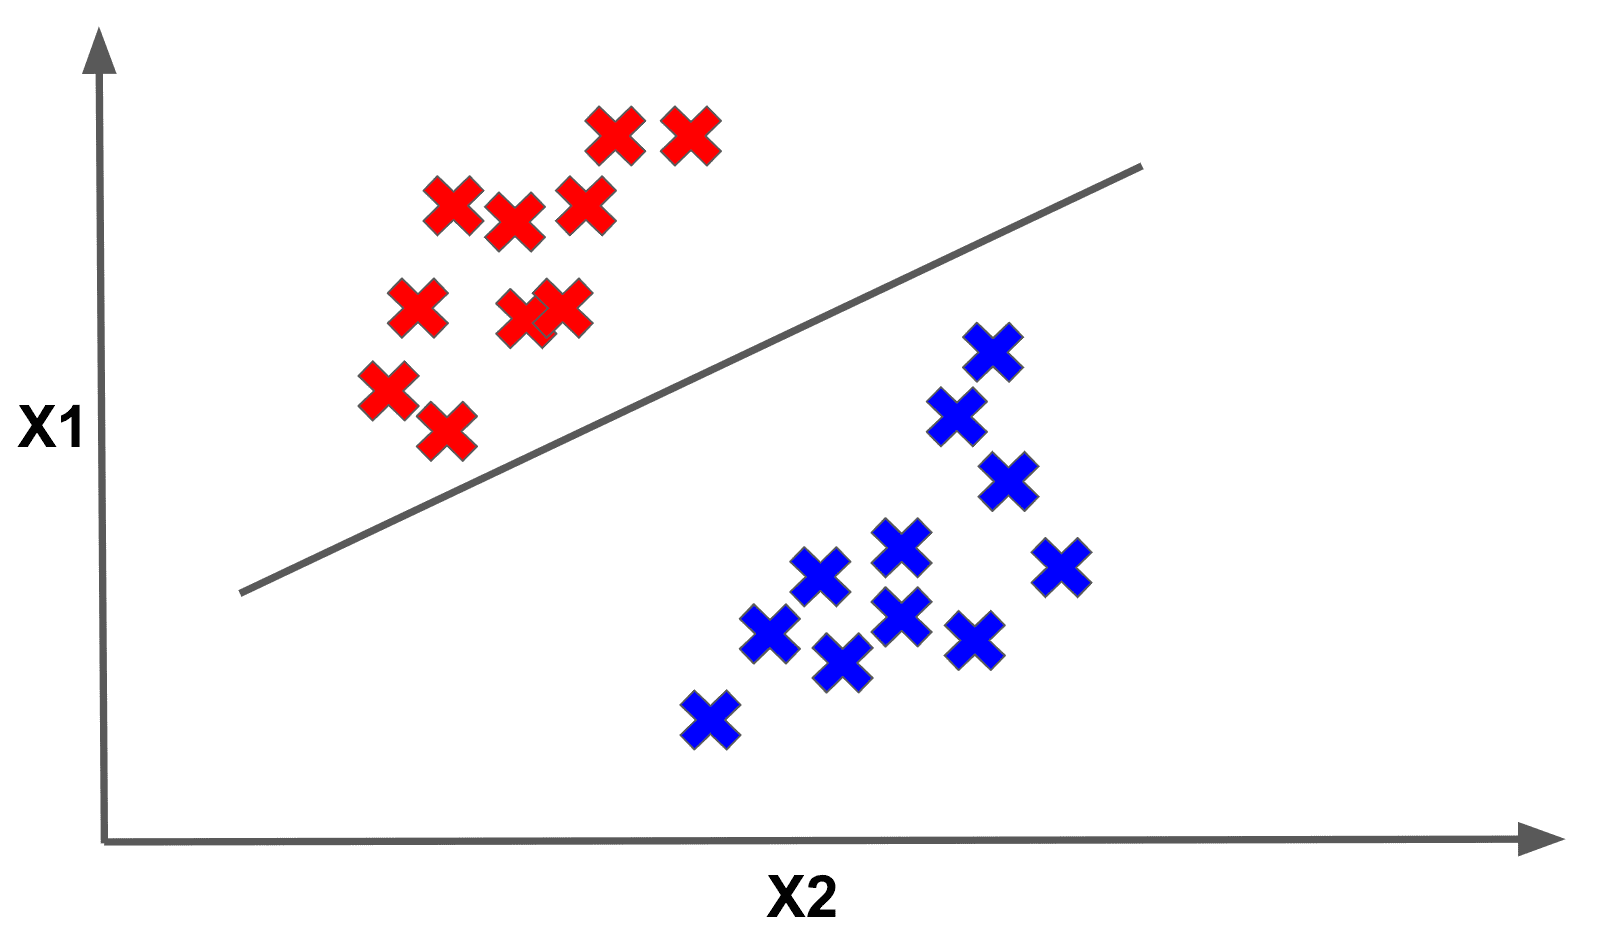
\includegraphics[width=\textwidth]{figures/2/linear_separator}
	\caption{\emph{Linear separator} is a vector-threshold pair \data{$(w, k)$} which can satisfy these 2 relations.}
	\label{fig:linear_separator}
\end{figure}

Binary \emph{classification} \data{$y_{i} \in \{-1, 1\}$} can be viewed as the task of \emph{separating classes} in feature space.

\begin{minipage}[m]{0.4\textwidth}
	\begin{figure}[H]
		\centering
		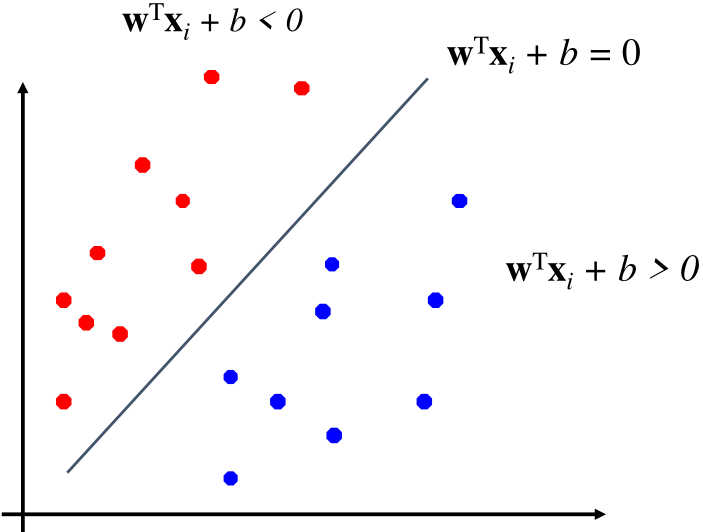
\includegraphics[width=\textwidth]{figures/2/linear_separator_2}
		\caption{Vectorized linear seperator.}
		\label{fig:linear_separator_2}
	\end{figure}
\end{minipage}\hfill%
\begin{minipage}[m]{0.6\textwidth}
	\begin{itemize}
		\item Hypothesis class of linear \emph{decision surfaces} is \data{$f(\vec{x}_{i}) = \sign(\vec{w}^{T}\vec{x}_{i} + b)$.}
		\item Without loss of generality, we assume that \data{$b=0$}.
		Thus, we get the simplified \data{$f(x_{i}) = \sign(\vec{w}^{T}\vec{x_{i}})$.}
		\item \data{$y_{i}(\vec{w}^{T}\vec{x}_{i}) > 0$} $\Leftrightarrow$ data point \data{$x_{i}$} is correctly \emph{classified.}
		\begin{itemize}
			\item Remember, \data{$y_{i}$} is counting as \data{1} or \data{-1}.
		\end{itemize}
	\end{itemize}
\end{minipage}

\section{Perceptron Algorithm}\label{sec:perceptron-algorithm}
\begin{itemize}
	\item Set time \data{$t=1$}, start with vector \data{$\vec{w}_{1}=\oldvec{0}$}.
	\item Given example \data{$\vec{x}$}, \emph{predict positive} iff (if and only if) \data{$\vec{w_{1}\cdot\vec{x} \geq 0}$}.
	\item On a mistake, update as follows:
	\begin{itemize}
		\item Mistake on \emph{positive}, then update \data{$\vec{w}_{t+1} \gets \vec{w}_{t} + \vec{x}$}.
		\item Mistake on \emph{negative}, then update \data{$\vec{w}_{t+1} \gets \vec{w}_{t} - \vec{x}$}.
	\end{itemize}
\end{itemize}

\subsection{Example}\label{subsec:perceptron-examplee}
\begin{table}[H]
	\centering
	\begin{tabular}{c c c c c}
		\data{$\vec{x}_{i}$:} & \textcolor{red}{$(1, 2)$} & \textcolor{red}{$(2, 3)$} & \textcolor{red}{$(2, 1)$} & \textcolor{red}{$(3, 0)$}\\
		\textcolor{blue}{$\vec{y}_{i}$:} & \textcolor{blue}{$+$} & \textcolor{blue}{$+$} & \textcolor{blue}{$-$} & \textcolor{blue}{$-$}\\
	\end{tabular}
\end{table}

\begin{minipage}[m]{0.6\textwidth}
	\data{\begin{equation*}
			  \begin{aligned}
				  \vec{w}_{1} &= [0\ 0]^{T}\\
				  \vec{w}_{1} \cdot \vec{x} &= [0\ 0]^{T} \cdot [1\ 2] = 0 \predict{+}{correct}\\
				  \vec{w}_{1} \cdot \vec{x} &= [0\ 0]^{T} \cdot [2\ 3] = 0 \predict{+}{correct}\\
				  \vec{w}_{1} \cdot \vec{x} &= [0\ 0]^{T} \cdot [2\ 1] = 0 \predict{+}{wrong}\\
				  \vec{w}_{2} &= \vec{w}_{1} - [2\ 1] = [-2\ -1]\\
				  \vec{w}_{2} \cdot \vec{x} &= [-2\ -1]^{T} \cdot [3\ 0] < 0 \predict{-}{correct}\\
				  \vec{w}_{2} \cdot \vec{x} &= [-2\ -1]^{T} \cdot [1\ 2] < 0 \predict{-}{wrong}\\
				  \vec{w}_{3} &= \vec{w}_{2} + [1\ 2] = [-1\ 1]\\
				  \vec{w}_{3} \cdot \vec{x} &= [-1\ 1]^{T} \cdot [2\ 3] > 0 \predict{+}{correct}\\
				  \vec{w}_{3} \cdot \vec{x} &= [-1\ 1]^{T} \cdot [2\ 1] < 0 \predict{-}{correct}\\
				  \vec{w}_{3} \cdot \vec{x} &= [-1\ 1]^{T} \cdot [3\ 0] < 0 \predict{-}{correct}\\
				  \vec{w}_{3} \cdot \vec{x} &= [-1\ 1]^{T} \cdot [1\ 2] > 0 \predict{+}{correct}\\
			  \end{aligned}
	\end{equation*}
	\begin{equation*}
	\begin{aligned}
		\vec{w}_{3} \cdot \vec{x} = [-1\ 1]^{T} \cdot [x_{1}\ x_{2}]
	\end{aligned}
	\end{equation*}}
	\textcolor{blue}{$-1x_{1} + 1x_{2} = 0$} is the linear separator.
\end{minipage}\hfill%
\begin{minipage}[m]{0.4\textwidth}
	\begin{figure}[H]
		\centering
		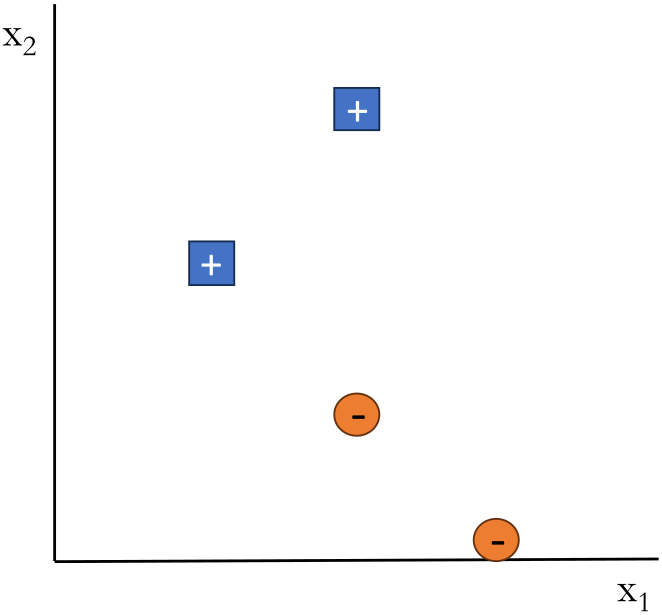
\includegraphics[width=\textwidth]{figures/2/perceptron_example}
		\caption{}
		\label{fig:perceptron_example}
	\end{figure}

\end{minipage}

\section{Geometric Margin}\label{sec:geometric-margin}
\begin{minipage}[m]{0.72\textwidth}
	The \emph{margin} of example $\data{\vec{x}}$ w.r.t (with respect to) a \emph{linear separator} \data{$\vec{w}$} is the distance from \data{$\vec{x}$} to the plane \data{$\vec{w}^{T} \cdot \vec{x} = 0$}.

	The \emph{margin} \data{$\gamma$} of a set of examples $\data{S}$ w.r.t a \emph{linear separator} \data{$\vec{w}$} is the largest margin over points \data{$\vec{x}\in S$}.
	Theorem: If the data has a \emph{margin} \data{$\gamma$} and all points lie inside a ball of \emph{radius} \data{$R$}, then the Perceptron algorithm makes \data{$\leq \frac{R}{\gamma^{2}}$} \emph{mistakes.}
\end{minipage}\hfill%
\begin{minipage}[m]{0.25\textwidth}
	\begin{figure}[H]
		\centering
		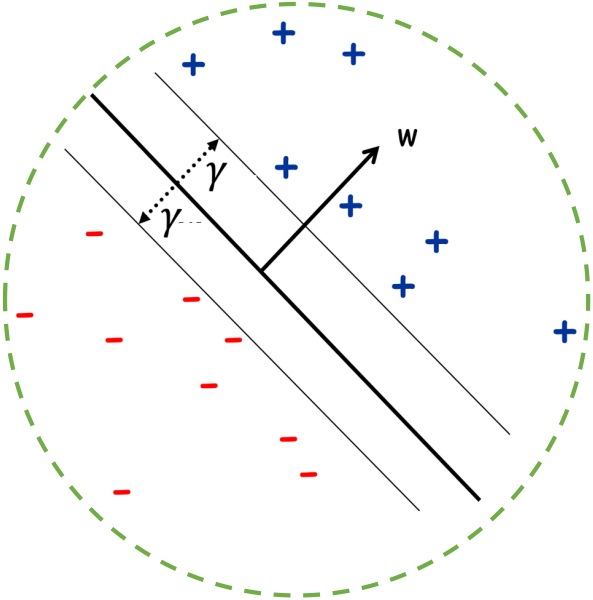
\includegraphics[width=\textwidth]{figures/2/geometric_margin}
		\caption{}
		\label{fig:geometric-margin}
	\end{figure}

\end{minipage}

\section{Support Vector Machine}\label{sec:svm}
\emph{Support vector machines} (SVMs) are \emph{supervised max-margin} models with associated learning algorithms.
\begin{itemize}
	\item Good \emph{generalization} in theory.
	\item Good \emph{generalization} in practice.
	\item Work well with \emph{few training instances}.
	\item Find \emph{globally best} model.
	\item \emph{Efficient algorithms}.
	\item Amenable to the \emph{kernel trick}.
\end{itemize}

\section{Optimal Linear Separator}\label{sec:optimal-linear-separator}
Which of the \emph{linear separators} is optimal?

\section{Classification Margin}\label{sec:classification-margin}
Examples closest to the hyperplane are \emph{support vectors}.
Margin \data{$\rho$} of the separator is the \emph{distance between support vectors}.

\begin{figure}[H]
	\centering
	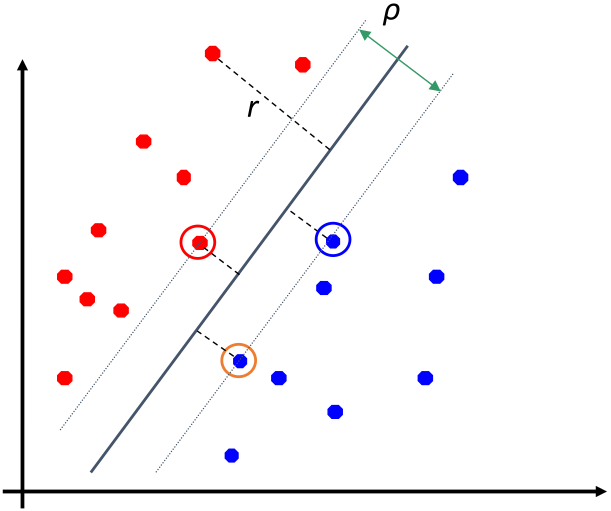
\includegraphics[width=0.5\textwidth]{figures/2/classification_margin}
	\caption{}
	\label{fig:classification-margin}
\end{figure}

\section{Maximizing the Margin}\label{sec:maximizing-the-margin}
\begin{itemize}
	\item Better \emph{Generalization} -- A larger margin allows the SVM to \emph{better generalize} to new, unseen data, leading to \emph{higher predictive accuracy}.
	\item Improved \emph{Robustness} -- A larger margin can lead to improved robustness \emph{against noise and outliers} in the training data, as it allows for \emph{greater tolerance} of misclassified examples.
	\item Reducing \emph{Overfitting} -- A larger margin can help \emph{reduce overfitting} by creating a \emph{simpler decision boundary} that is less sensitive to small fluctuations in the training data.
	\item Enhanced \emph{Interpretability} -- A larger margin can lead to clearer and more \emph{interpretable decision boundaries}, making it easier to understand the model's behavior.
\end{itemize}

\section{Linear SVM}\label{sec:linear-svm}
Let training set \data{$\left\{ (\vec{x}_{i}, y_{i})_{i=1\dots{}n}\ , \vec{x}_{i}\in\mathbb{R}^{d}, y_{i} \in \{ -1, 1\} \right\}$} be separated by a hyperplane with margin \data{$\rho$}.
Then for each training example \data{$(\vec{x}_{i}, y_{i})$}

\data{\begin{equation*}
\begin{aligned}
	\vec{w}^{T}\vec{x}_{i} + b \geq 1 && \mbox{ if } y_{i} = 1 &&\\
	&&&& \Leftrightarrow y_{i}\left( \vec{w}^{T}\vec{x}_{i} + b \right) \geq 1\\
	\vec{w}^{T}\vec{x}_{i} + b \leq -1 && \mbox{ if } y_{i} = -1 &&\\
\end{aligned}
\end{equation*}}

Geometrically, the \emph{distance} between the \emph{2 hyperplanes} can be expressed as:
\data{\begin{equation}
	\rho = \frac{2}{||w||}
	\label{eq:hyperplane-distance}
\end{equation}}

Then we can formulate the \emph{quadratic optimization problem}:

\begin{svmbox}
	Find \data{$\vec{w}$} and \data{$b$} such that \data{\[ \rho = \frac{2}{||\vec{w}||} \]} is \emph{maximized} \emph{and} for all \data{$\left( \vec{x}_{i}, y_{i} \right), i=1\dots{}n : y_{i}\left( \vec{w}^{T}\vec{x}_{i} + b \right) \geq 1$}
\end{svmbox}

Which can be reformulated as:

\begin{svmbox}
	\data{$\forall(\vec{x}_{i}, y_{i})$}, find \data{$\vec{w}$} and \data{$b$} such that
	\data{\[ \mbox{\emph{Minimize }} Q(w) = \frac{1}{2}||\vec{w}||^{2} = \frac{1}{2}\vec{w}^{T}\vec{w} \]}
	subject to \data{$y_{i}(\vec{w}^{T}\vec{x}_{i} + b) \geq 1,\ \ \forall i \in [1, n]$}
\end{svmbox}

\section{Lagrangian Duality}\label{sec:lagrangian-duality}
\begin{itemize}
	\item Need to \emph{optimize} a \emph{quadratic function} subject to \emph{linear constraints}.
	\item Quadratic optimization problems are a well-known class of mathematical programming problems for which several (non-trivial) algorithms exist.
	\item Solution involves \emph{constructing dual problem} where \emph{Lagrange multipliers} \data{${\alpha_{i}}$} is associated with all inequality constraint in primal (original) problem:
\end{itemize}

\begin{svmbox}
	\data{$\forall i$}, find \data{$\alpha_{1}, \alpha_{2}, \dots, \alpha_{n}$} such that
	\data{\[ \mbox{\emph{Minimize} } Q(\alpha) = \sum_{i}\alpha_{i} - \frac{1}{2}\sum_{i}\sum_{j} \alpha_{i} \alpha_{j} y_{i} y_{j} \vec{x}_{i}^{T} \vec{x}_{j} \]}
	subject to \data{$\alpha_{i} \geq 0$}
\end{svmbox}

Minimize \data{$\frac{1}{2}\vec{w}^{T}\vec{w}$} s.t.\ (subject to) \data{$1 - y_{i} (\vec{w}^{T}\vec{x}_{i} + b) \leq 0,\ \ \forall i \in [1, n] $}

The Lagrangian \data{$\mathcal{L} = \frac{1}{2}\vec{w}^{T}\vec{w} + \sum_{i}\alpha_{i} (1 - y_{i}(\vec{w}^{T}\vec{x}_{i} + b )) $}
\data{\begin{equation*}
\begin{aligned}
	\frac{\partial \mathcal{L}}{\partial w} &= 0\\
	\vec{w} + \sum_{i} \alpha_{i} (-y_{i})\vec{x}_{i} &= 0\\
	\vec{w} &= \sum_{i} \alpha_{i} y_{i} \vec{x}_{i}
\end{aligned}
\end{equation*}
\begin{equation*}
\begin{aligned}
	\frac{\partial \mathcal{L}}{\partial b} &= 0\\
	\sum_{i} \alpha_{i}y_{i} &= 0
\end{aligned}
\end{equation*}}

Substituting \data{$\vec{w} = \sum_{i} \alpha_{i} y_{i} \vec{x}_{i}$} into \data{$\mathcal{L}$}

\data{\begin{equation*}
\begin{aligned}
	\mathcal{L} &= \frac{1}{2} \left( \sum_{i} \alpha_{i} y_{i} \vec{x}_{i} \right)^{T}\left( \sum_{i} \alpha_{i} y_{i} \vec{x}_{i} \right) + \sum_{i}\alpha_{i}\left( 1 - y_{i} \left( \sum_{j} \alpha_{j} y_{j} \vec{x}_{j}^{T}\vec{x}_{i} + b\right) \right)\\
				&= \frac{1}{2} \sum_{i}\sum_{j} \alpha_{i} \alpha_{j} y_{i} y_{j} \vec{x}_{i}^{T} \vec{x}_{j} + \sum_{i}\alpha_{i} - \sum_{i} \sum_{j} \alpha_{i} \alpha_{j} y_{i} y_{j} \vec{x}_{j}^{T}\vec{x}_{i} + b \left( \sum_{i} a_{i} y_{i} \right)\\
				&= -\frac{1}{2}\sum_{i}\sum_{j} \alpha_{i} \alpha_{j} y_{i} y_{j} \vec{x}_{i}^{T} \vec{x}_{j} + \sum_{i} \alpha_{i}
\end{aligned}
\end{equation*}}
\begin{itemize}
	\item The \emph{new objective function} is in terms of \data{$a_{i}$} only.
	\item The original problem is known as the primal problem.
	\item The objective function of the \emph{dual} problem needs to be \emph{maximized}.
\end{itemize}

\section{SVM Solution}\label{sec:svm-solution}
\begin{itemize}
	\item Given a \emph{solution} \data{$a_{1}\dots a_{n}$} to the dual problem, solution to the primal is:
	\begin{svmbox}
		\data{\[ \vec{w} = \sum a_{i}y_{i}\vec{x}\ \ \ b = y_{k} - \sum a_{i}y_{i}\vec{x}_{i}^{T}\vec{x}_{k} \mbox{ for any } a_{k} > 0  \]}
	\end{svmbox}
	\item Each non-zero \data{$a_{i}$} indicates that corresponding \data{$\vec{x}_{i}$} is a \emph{support vector}.
	\item Then the \emph{classifying function is:}
	\begin{svmbox}
		\[ \data{ f(x) = \sum a_{i}y_{i}\vec{x}_{i}^{T}\vec{x} + b } \]
	\end{svmbox}
	\item Notice that it relies on the \emph{inner product} between the test point \data{$\vec{x}$} and the support vectors \data{$\vec{x}_{i}$}.
	\item Solving the optimization problem involves \emph{computing the inner products} \data{$\vec{x}_{i}^{T}\vec{x}_{j}$} between all training points.
\end{itemize}

\section{Soft Margin Classification}\label{sec:soft-margin-classification}
\begin{itemize}
	\item What if the training set is \emph{not linearly separable?}
	\item \emph{Slack variables} \data{$\xi_{i}$} can be added to \emph{allow misclassification} of difficult or noisy examples; thus, the result margin is called \emph{soft}.
\end{itemize}
\begin{figure}[H]
	\centering
	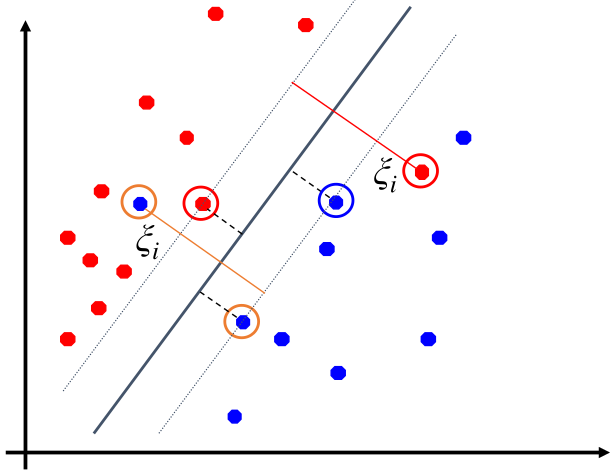
\includegraphics[width=0.5\textwidth]{figures/2/soft_margin_classification}
	\caption{}
	\label{fig:soft-margin-classification}
\end{figure}

\begin{svmbox}
	\data{$\forall (\vec{x}_{i}, y_{i})$}, find \data{$\vec{w}$} and \data{$b$} such that
	\[ \mbox{\emph{Minimize} } \data{ Q(\vec{w}, \xi_{i}) = \frac{1}{2}\vec{w}^{T}\vec{w} + C\sum_{i=1}^{n}\xi_{i} } \]
	subject to \data{$\xi_{i} \geq 0$} and \data{$y_{i}(\vec{w}^{T}\vec{x}_{i} + b) \geq 1 - \xi_{i},\ \ \forall i \in [1,n]$}
\end{svmbox}

The \emph{tradeoff} between the \emph{maximization} of the \emph{margin} and \emph{minimization} of the \emph{classification error} is determined by the margin \emph{parameter} \data{$C$}.

\section{Soft Margin SVM Solution}\label{sec:soft-margin-svm-solution}
\begin{svmbox}
	\data{$\forall i$}, find \data{$\alpha_{1} \dots \alpha_{n}$} such that
	\[ \mbox{\emph{Maximize} } \data{ Q(a) = \sum_{i}\alpha_{i} = \frac{1}{2}\sum_{i} \sum_{j} \alpha_{i} \alpha_{j} y_{i} y_{j} \vec{x}_{i}^{T} \vec{x}_{j} } \]
	subject to \data{$0 \leq \alpha_{i} \leq C$} and \data{$\sum_{i} \alpha_{i} y_{i} = 0$}
\end{svmbox}

The solution is:
\begin{svmbox}
	\[ \data{ \vec{w} = \sum \alpha_{i} y_{i} \vec{x}_{i}\ \ \ \ b = y_{k}(1 - \xi_{i}) - \sum \alpha_{i} y_{i} \vec{x}_{i}^{T} \vec{x}_{k} \mbox{   for any } \alpha_{k} > 0 } \]
\end{svmbox}

\section{Kernel Method}\label{sec:kernel-method}
\begin{itemize}
	\item If we \emph{map} the \emph{input vectors} into a very \emph{high-dimensional feature space}, the task of \emph{finding} the \emph{maximum-margin separator} can become \emph{computationally intractable}.
	\item All of the \emph{computations} that we need to do to find the \emph{maximum-margin separator} (SVM optimization problem) can be expressed in terms of \emph{inner products} between \emph{pairs of data points} (in the high-dimensional feature space).
	\item These \emph{inner products} are the only part of the computation that depends on the dimensionality of the high-dimensional space.
	So, if we had a \emph{fast way} to do the dot products, we would \emph{not have to pay a price} for solving the learning problem in the high-dimensional space.
	\item The \emph{kernel trick} is just a way of \emph{doing inner products} a whole lot faster than is usually possible.
	It relies on \emph{choosing a way of mapping} to the \emph{high-dimensional feature space} that allows fast scalar products.
	\item By using a \emph{nonlinear vector function} \data{$\phi(x) = \left< \phi(\vec{x}_{1}), \dots, \phi(\vec{x}_{n}) \right>$}, the \data{$n$}-dimensional input vector \data{$\vec{x}$} can be mapped into high-dimensional feature space.
	The \emph{decision function} in the feature space is expressed as:
	\[ \data{ f(x) = \vec{w}^{T}\phi(\vec{x}) + b } \]
	\item In terms of solving the \emph{quadratic optimization problem of SVM}, each training data point is in the form of dot products.
	A \emph{kernel function} \data{$K$} simplifies the calculation of dot product terms \data{$\left< \phi(\vec{x}_{i}) \cdot \phi(\vec{x}_{j}) \right>$}.
	\[ \data{K(\vec{x}_{i}, \vec{x}_{j}) = \phi(\vec{x}_{i})^{T} \phi(\vec{x}_{j})} \]
\end{itemize}

\begin{table}[H]
	\centering
	\caption{Kernel Functions}
	\label{tab:kernel-fucntions}
	\begin{tabular}{|c|c|c|}
		\hline
		\textbf{Kernel Name} & \textbf{Category} & \textbf{Kernel Function}\\
		\hline
		Polynomial & Global & $K(\mu, v) = (\mu \cdot v + 1)^{d}$\\
		\hline
		Radial Basis Kernel (RBF) & Local & $K(\mu, v) = \exp( -\gamma || \mu - v ||^{2} )$\\
		\hline
	\end{tabular}
\end{table}

\begin{minipage}[m]{0.55\textwidth}
	\begin{figure}[H]
		\centering
		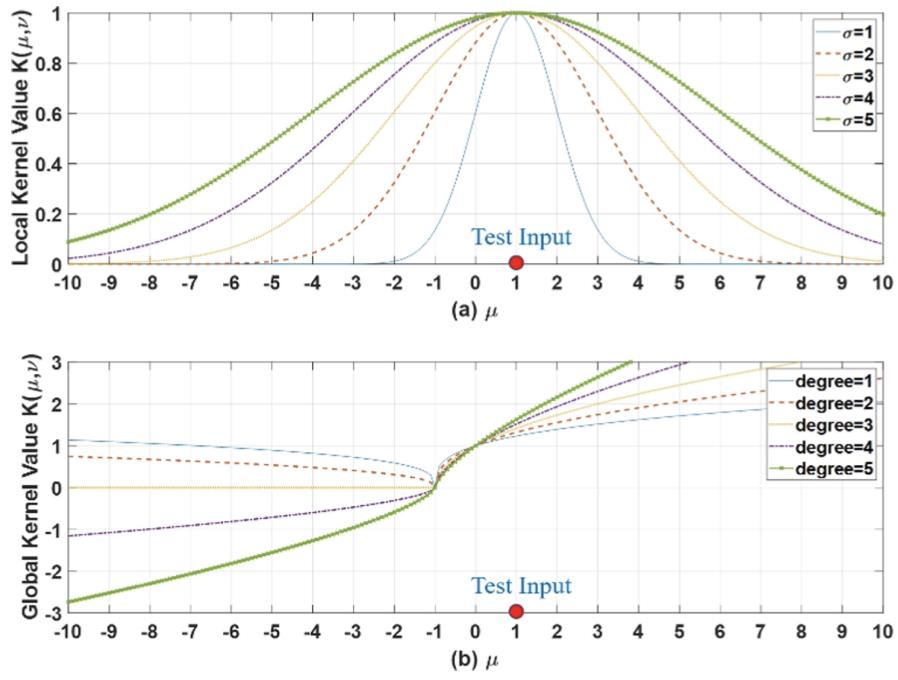
\includegraphics[width=\textwidth]{figures/2/kernels}
		\caption{}
		\label{fig:kernel-graphs}
	\end{figure}
	
\end{minipage}\hfill%
\begin{minipage}[m]{0.45\textwidth}
	\subsection{Local Kernels}\label{subsec:local-kernels}
	\begin{itemize}
		\item Only \emph{nearby data points} affect SVM model.
		\item Has \emph{higher learning} ability, but the \emph{generalization} ability is \emph{lower}.
		\item Used when there is \emph{no prior knowledge} about the training dataset.
	\end{itemize}

	\subsection{Global Kernels}\label{subsec:global-kernels}
	\begin{itemize}
		\item \emph{Data points} from \emph{greater distance} can affect SVM\@.
		\item Has a \emph{higher generalization ability}, but the \emph{learning} ability is \emph{lower}.
	\end{itemize}
\end{minipage}

\section{Kernel Functions}\label{sec:kernel-functions}
Linear:
\data{\begin{equation}
	K(\vec{x}_{i}, \vec{x}_{j}) = \vec{x}_{i} \cdot \vec{x}_{j}
	\label{eq:linear-kernel}
\end{equation}}

Polynomial:
\data{\begin{equation}
	K(\vec{x}_{i}, \vec{x}_{j}) = \left(1 + \vec{x}_{i} \cdot \vec{x}_{j} \right)^{p}
	\label{eq:polynomial-kernel}
\end{equation}}

Gaussian (Radial Basis Function):
\data{\begin{equation}
	K(\vec{x}_{i}, \vec{x}_{j}) = e^{\left( \frac{-|| \vec{x}_{i} - \vec{x}_{j} ||^{2}}{2\sigma^{2}} \right)}
	\label{eq:gaussian-kernel}
\end{equation}}

Laplace:
\data{\begin{equation}
	K(\vec{x}_{i}, \vec{x}_{j}) = e^{\left( \frac{-|| \vec{x}_{i} - \vec{x}_{j} ||}{2\sigma^{2}} \right)}
	\label{eq:laplace-kernel}
\end{equation}}

Sigmoid:
\data{\begin{equation}
	K(\vec{x}_{i}, \vec{x}_{j}) = \tanh\left( \kappa (\vec{x}_{i} \cdot \vec{x}_{j}) + \sigma \right)
	\label{eq:sigmoid-kernel}
\end{equation}}

\section{Kernel Trick}\label{sec:kernel-trick}
\begin{itemize}
	\item The linear classifier~\eqref{eq:linear-kernel} relies on the \emph{inner product} between vectors.
	\[ \data{ K(\vec{x}_{i}, \vec{x}_{j}) = \vec{x}_{i}^{T}\vec{x}_{j} } \]
	\item If \emph{every data point} is \emph{mapped} into \emph{high-dimensional space} via some transformation \data{$\mathbf{\phi}: x \rightarrow \phi(x)$}, the inner product becomes --
	\[ \data{ K(\vec{x}_{i}, \vec{x}_{j}) = \phi(\vec{x}_{i})^{T}\phi(\vec{x}_{j}) } \]
	\item A \emph{kernel function} is a function that is equivalent ot an inner product in some feature space.
	As long as we can \emph{calculate the inner product in the feature space}, we do \emph{not} need to compute each \data{$\phi(x)$} explicitly.
\end{itemize}

Example: Take this 2-dimensional vector: \data{$\vec{x} = [x_{1}, x_{2}]$}
\data{\begin{equation*}
	\begin{aligned}
		K(\vec{x}_{i}, \vec{x}_{j}) &= (1 + \vec{x}_{i}^{T}\vec{x}_{j})^{2}\\
		&= 1 + x_{i1}^{2}x_{j1}^{2} + 2x_{i1}x_{j1}x_{i2}x_{j2} + x_{i2}^{2}x_{j2}^{2} + 2x_{i1}x_{j1} + 2x_{i2}x_{j2}\\
		&= \left[ 1\ \ x_{i1}^{2}\ \ \sqrt{2}x_{i1}x_{i2}\ \ x_{i2}^{2}\ \ \sqrt{2x_{i1}}\ \ \sqrt{2x_{i2}} \right]^{T} \left[ 1\ \ x_{j1}^{2}\ \ \sqrt{2}x_{j1}x_{j2}\ \ x_{j2}^{2}\ \ \sqrt{2x_{j1}}\ \ \sqrt{2x_{j2}} \right]\\
		&= \phi(\vec{x}_{i})^{T}\phi(\vec{x}_{j})
	\end{aligned}
\end{equation*}}
where \data{$\phi(\vec{x}) = \left[ 1\ \ x_{1}^{2}\ \ \sqrt{2}x_{1}x_{2}\ \ x_{2}^{2}\ \ \sqrt{2x_{1}}\ \ \sqrt{2x_{2}} \right]^{T}$}

This use of the \emph{kernel function} to \emph{avoid} computing \data{$\phi(x)$} explicitly is known as the \emph{kernel trick}.

\section{Determining Kernels}\label{sec:determining-kernels}
For some \emph{functions} \data{$K(\vec{x}_{i}, \vec{x}_{j})$} checking that \data{$K(\vec{x}_{i}, \vec{x}_{j}) = \phi(\vec{x}_{i})^{T}\phi(\vec{x}_{j})$} can be cumbersome.\\

\subsection{Mercer's theorem}\label{subsec:mercers-theorem}
\begin{itemize}
	\item \data{$K$} is a \emph{kernel} iff:
	\begin{itemize}
		\item \data{$K$} is \emph{symmetric} i.e., \data{$K = K^{T}$}.
		\item \data{$K$} is \emph{positive semi-definite} i.e., \data{$c^{T}Kc \geq 0$}, where \data{$c \in \mathbb{R}$} is a vector.
	\end{itemize}
\end{itemize}

\section{Non-linear SVMs}\label{sec:non-linear-svms}
\begin{svmbox}
	\data{$\forall i$}, find \data{$\alpha_{1} \dots \alpha_{n}$} such that
	\[ \mbox{\emph{Maximize} } Q(a) = \sum_{i}\alpha_{i} - \frac{1}{2} \sum_{i} \sum_{j} \alpha_{i} \alpha_{j} y_{i} y_{j} K(\vec{x}_{i}, \vec{x}_{j}) \]
	subject to \data{$\alpha_{i} \geq 0$} and \data{$\sum_{i} \alpha_{i}y_{i} = 0$}.
\end{svmbox}

The solution is:
\data{\begin{equation}
	f(\vec{x}) = \sum \alpha_{i} y_{i} K(\vec{x}_{i}, \vec{x}_{j}) + b
	\label{eq:non-linear-svms}
\end{equation}}


\begin{figure}[H]
	\centering
	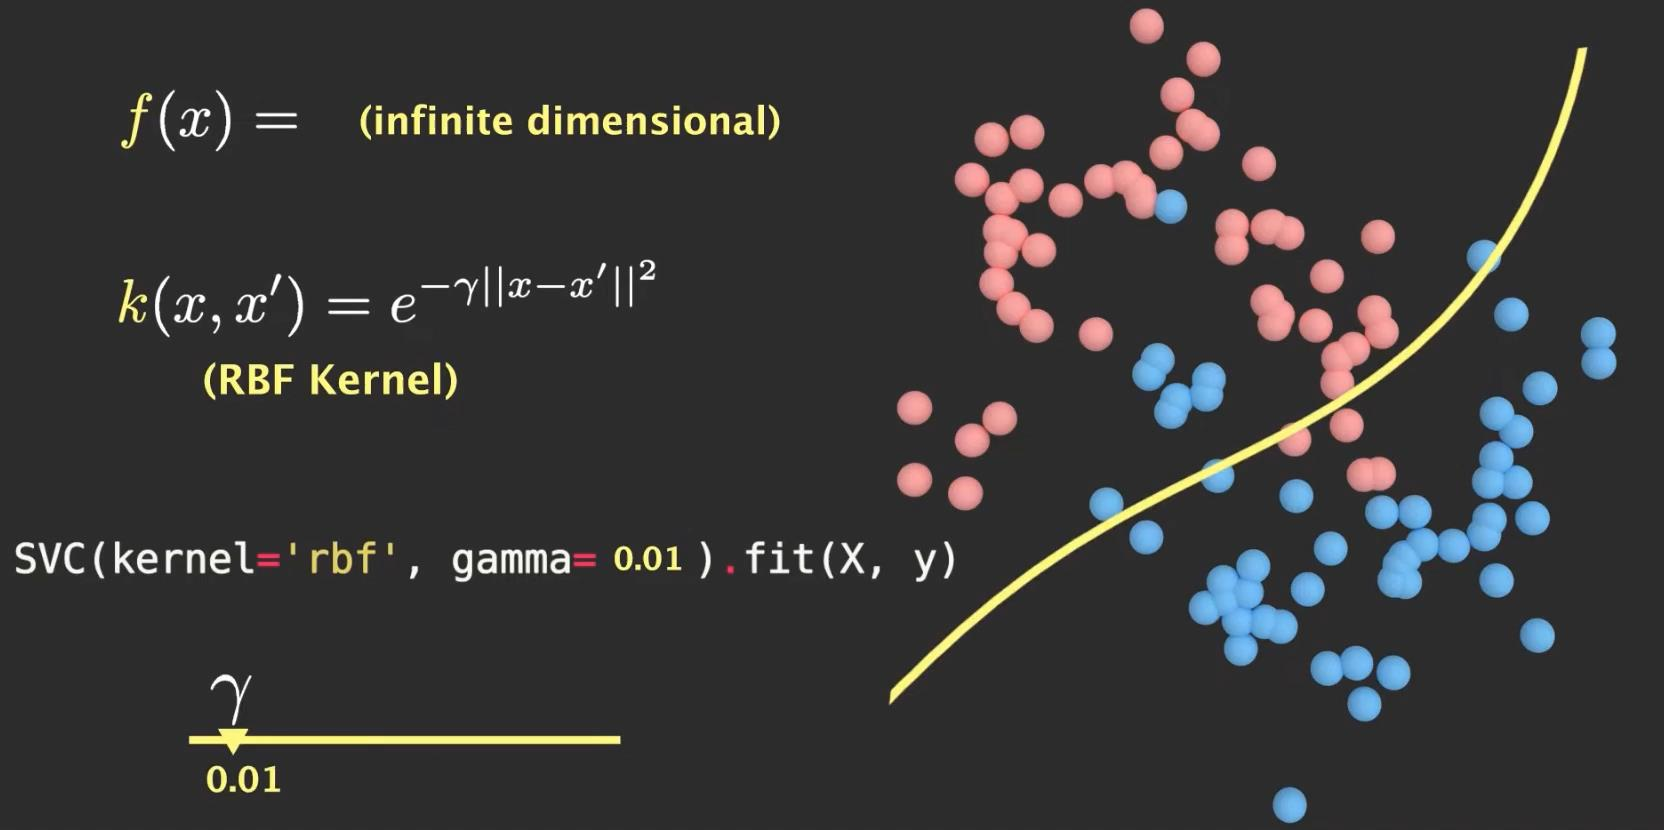
\includegraphics[width=\textwidth]{figures/2/infinite-dimension}
	\caption{}
	\label{fig:infinite-dimension}
\end{figure}


\section{Kernel Closure Properties}\label{sec:kernel-closure-properties}
\begin{itemize}
	\item Easily \emph{create new kernels} using basic ones.
	\item If \data{$K_{1}(\cdot, \cdot)$} and \data{$K_{2}(\cdot, \cdot)$} are kernels and \data{$c_{1} \geq 0$}, \data{$c_{2} \geq 0$}, then --
	\begin{itemize}
		\item \data{$K = c_{1}K_{1} + c_{2}K_{2}$} is a kernel,
		\item \data{$K = K_{1}K_{2}$} is a kernel.
	\end{itemize}
\end{itemize}

\section{Kernel Benefits}\label{sec:kernel-benefits}
\begin{itemize}
	\item Offers great \emph{modularity}.
	\item \emph{No need} to \emph{change} the \emph{underlying learning algorithm} to \emph{accommodate} a particular choice of kernel function.
	\item Can \emph{substitute} a \emph{different algorithm} while maintaining the \emph{same kernel}.
\end{itemize}

\section{Conclusion}\label{sec:conclusion}
Strengths:
\begin{itemize}
	\item Fast.
	\item Training is relatively easy.
	\item It scales relatively well high dimensional data.
	\item Tradeoff between classifier complexity and error can be controlled explicitly.
	\item Non-traditional data like strings and trees can be used as input to SVM, instead of feature vectors.
\end{itemize}

Weaknesses:
\begin{itemize}
	\item Need to choose a ``good'' kernel function.
\end{itemize}

\end{document}
